\documentclass{article}
\usepackage{graphicx} % Required for inserting images
\input{setup}
\usepackage{polski}
\usepackage[margin=2cm]{geometry}
\title{Wyznaczanie stanów dwuelektronowych metodą czasu urojonego i~Hartree--Focka}
\author{Marta Wleklińska}
\date{\today}

\begin{document}

\maketitle

\section{Wstęp}
W poniższym ćwiczeniu opisywany będzie układ dwóch elektronów uwięzionych w kropce kwantowej.
Jedną z metod opisu stanu takiego układu jest metoda czasu urojonego.
Polega ona na podstawieniu w równaniu Schr{\"o}dingera zależnym od czasu czasu $t = \ii \tau$.
Otrzymujemy zatem iteracyjną wartość kolejnych wartości $\Psi^{(k+1)}$
\begin{equation}
    \Psi^{(k+1)} = \left(1 - \Delta \tau \mathbf{\hat{H}}\right)\Psi^{(k)}.
\end{equation}
Procedura znajdowania funkcji falowej oraz odpowiadających jej energii bazuje na tym iteracyjnym wzorze.
Pochodna przestrzenna w części kinetycznej operatora Hamiltona~$\mathbf{\hat{H}}$ przybliżana jest ilorazem różnicowym.
Następnie przeprowadzana jest normalizacja, obliczana energia oraz porównywana do przyjętej wartości krytycznej tolerancji.\\
\\
Inną z metod, która pozwala na badanie układu jest metoda Hartree--Focka.
Kluczową składową otrzymaną w wyprowadzeniach metody jest operator Focka $\mathbf{\hat{F}}(x_i)$, który w ogólnym przypadku składa się z czynnika hamiltonianu jednoelektronowego oraz różnicy operatorów kulobowskiego (oraz wymiany), które kolejno są dane zależnościami
\begin{gather}
    \mathbf{\hat{h}} \psi_{1i} = \frac{-1}{2m^*}\frac{\psi_{1i+1} + \psi_{1i-1}-2\psi_{1i}}{\Delta x^2}, \quad i = 1, ..., n-2,\\
    \mathbf{\hat{J}}\psi_{1} = \left[\sum_{j=1}^{n-1}V_{\text{int}}\left(x_i - x_j\right)|\psi_{1j}|^2\Delta x\right]\psi_{1i}, \quad i = 1, ..., n-2,
\end{gather}
przy czym $V_{\text{int}}(\cdot, \cdot)$ jest potencjałem oddziaływania elektron--elektron.
Ponownie, liczony będzie operator Focka uzyskując wartość energii i będzie sprawdzana jest wartość wobec wartości tolerancji.
\section{Cel ćwiczenia}
Ćwiczenie polega na symulacji 2 elektronów uwięzionych w nieskończonej studni potencjału.
Metodą czasu urojonego wyznaczona zostanie zależność energii w funkcji liczby iteracji oraz jak elektrony zachowują się (rozkład) w zależności od wielkości kropki.
Dodatkowo, posługując się metodą Hartree--Focka wyznaczymy wartości energii w zależności od rozmiaru kropki ($30-60$~nm) oraz porównamy te wyniki z metodą czasu urojonego.

\section{Wyniki}
Pierwsza część ćwiczenia bazowała na implementacji metody czasu urojonego.
Jako sprawdzanie poprawności implementacji oraz zbadanie, jaki krok czasowy jest najbardziej optymalny, wyznaczona została zależność energii od liczby iteracji.
Na rysunku~\ref{fig:ex1} została przedstawiona na zależność.
\begin{figure}[htp!]
    \centering
    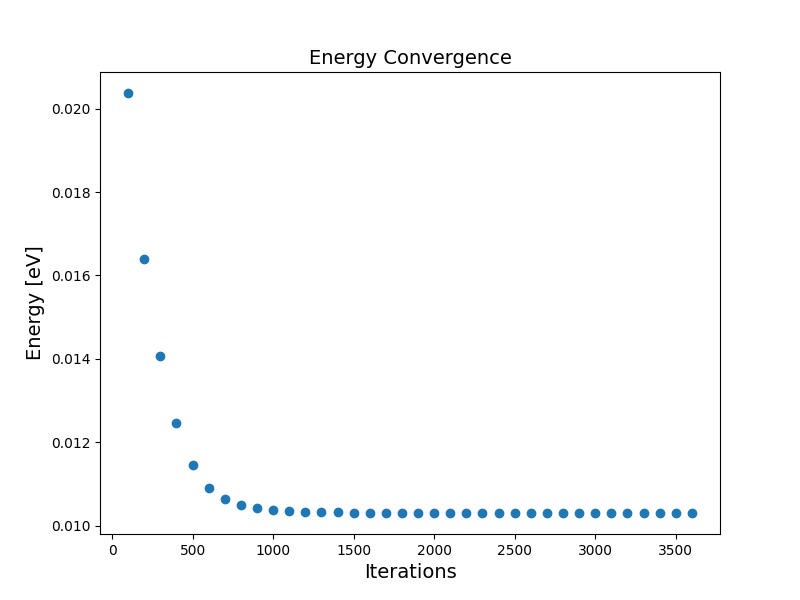
\includegraphics[width=0.75\linewidth]{ex1_energy_convergence.png}
    \caption{Energia uzyskana metodą czasu urojonego w funkcji kroku iteracji}
    \label{fig:ex1}
\end{figure}
Przy mniejszej liczbie iteracji $(<600)$ wartość energii maleje wykładniczo aż do wartości $\sim 600$ iteracji, po której wartość energii nie zmienia się znacznie.\\
\\
Oprócz energii, uzyskaliśmy funkcję falową, za pomocą której możemy uzyskać rozkład gęstości prawdopodobieństwa.
Oczywiście w zależności od tego, jaki jest rozmiar kropki, oddziaływania i mapa będzie wyglądać inaczej, zatem przyjęliśmy dwie różne wartości wielkości układu $a = \{30, 60\}$~nm.
Na rysunku~\ref{fig:rozmiary kropek} zostały przedstawione mapy rozkładu prawdopodobieństwa kropek o różnych rozmiarach.
\begin{figure}[htp!]
    \centering
\begin{subfigure}{.49\textwidth}
    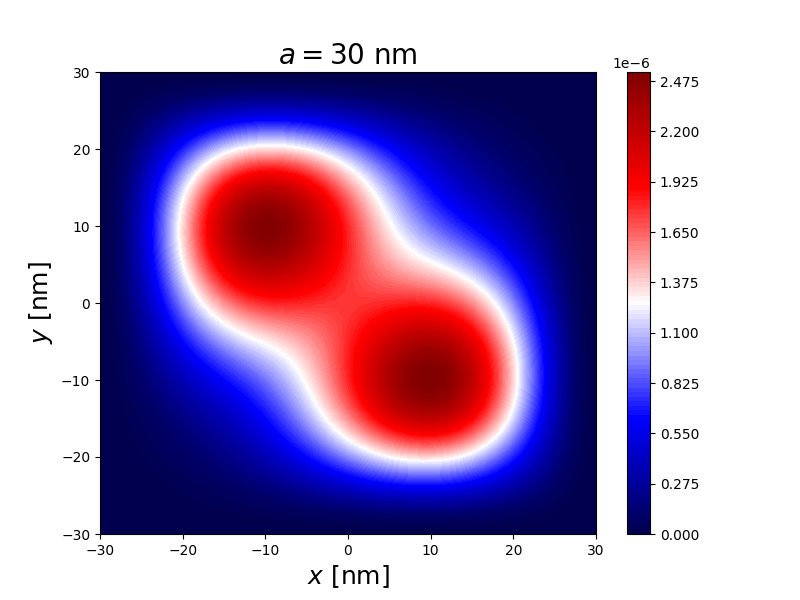
\includegraphics[width=1.0\linewidth]{ex2_$a = 30$ nm.png}
    \caption{}
    \label{fig:ex3:30cm}
\end{subfigure}
\begin{subfigure}{.49\textwidth}
    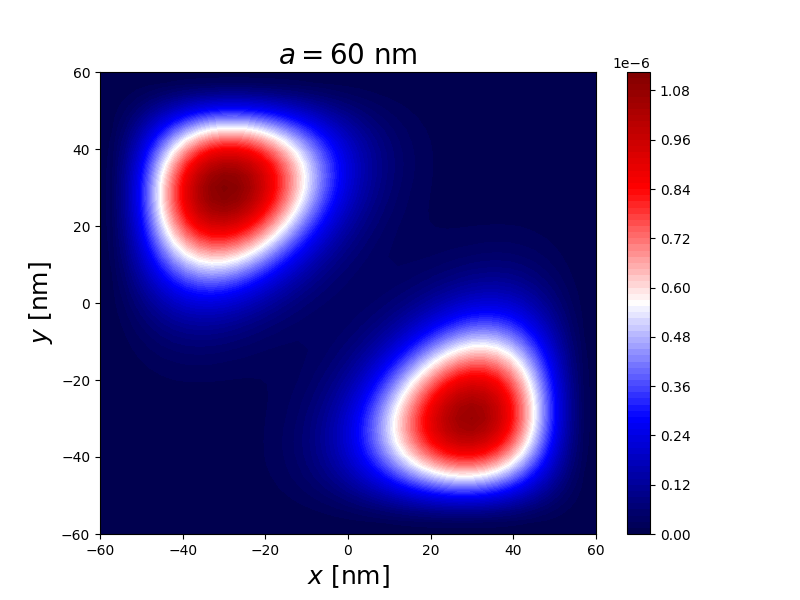
\includegraphics[width=1.0\linewidth]{ex2_$a = 60$ nm.png}
    \caption{}
    \label{fig:ex3:60 mm}
\end{subfigure}
\caption{Rozkład gęstości prawdopodobieństwa kropek kwantowych przy różnych rozmiarach układu: \textbf{(a)}~$a = 30$~nm; \textbf{(b)}~$a = 60$~nm}
\label{fig:rozmiary kropek}
\end{figure}
Wyraźnie na tych rozkładach widzimy różnice wynikające z wielkości poszczególnych układów.
Dla rysunku~\ref{fig:ex3:30cm}, w którym rozmiar układu jest mniejszy, rozkłady kolejnych elektronów nachodzą na siebie, podczas gdy w przypadku większego układu~(rys.~\ref{fig:ex3:60 mm}), wyraźnie widzimy oddzielenie większych wartości rozkładu gęstości prawdopodobieństwa znalezienia każdego z elektronów.

\subsection{Porównanie metody czasu urojonego i Hartree--Focka}
Ostatnia część ćwiczenia polegała na znalezieniu zależności energii układu w zależności od rozmiaru układu.
Wartości energii były wyznaczane dwoma metodami: metodą czasu urojonego oraz metodą Hartree--Focka.
Na rysunku~\ref{fig:comparison hf it} zostało przedstawione porównanie wyników tymi dwoma metodami.
\begin{figure}[htp!]
    \centering
    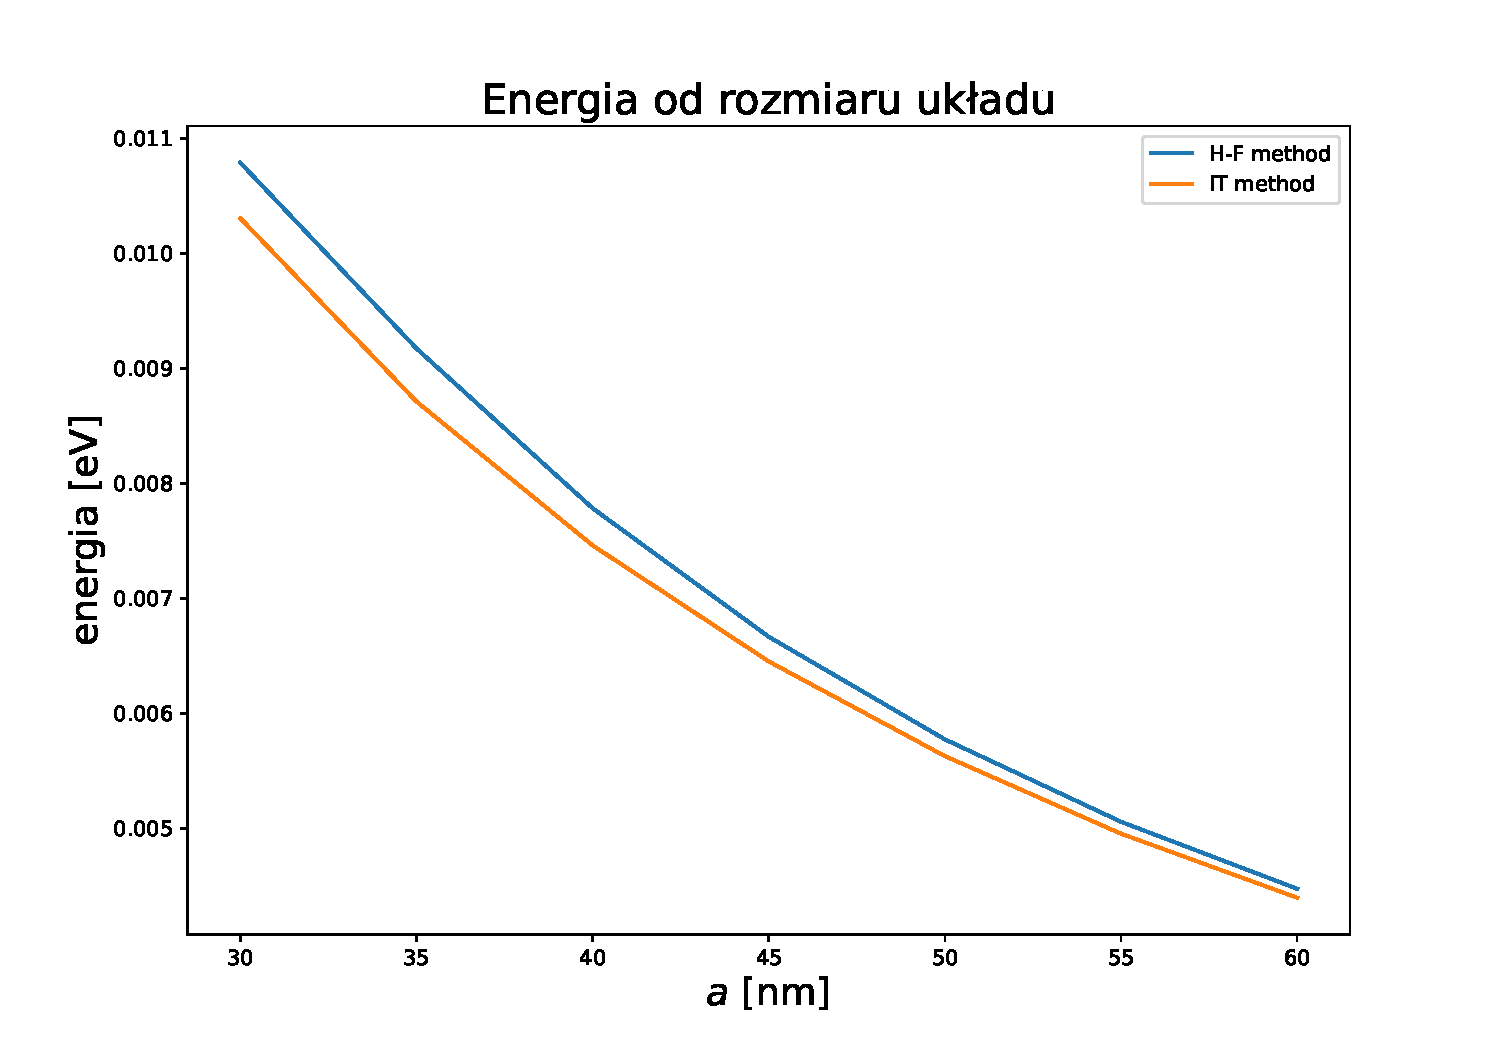
\includegraphics[width=0.75\linewidth]{ex2_4_energies.pdf}
    \caption{Porównanie metody czasu urojonego i Hartree--Focka przy znajdowaniu zależności energii od rozmiaru układu}
    \label{fig:comparison hf it}
\end{figure}
Zauważmy, że dla każdej wartości $a$, energia uzyskana metodą Hartree–Focka jest większa od tej uzyskanej metodą czasu urojonego. 
Przybliżenie jednoelektronowe w metodzie Hartree--Focka nie uwzględnia dynamicznych korelacji między elektronami.
Energia korelacji $E_{\text{corr}}$, którą należałoby uwzględnić w~ostatecznym wyniku jest różnicą energii dokładnej układu $E_0$ a tą uzyskaną w metodzie Hartree--Focka $E_{\text{H-F}}$, i.e.
\begin{gather}
    E_{\text{corr}} = E_0 - E_{\text{H-F}}.
\end{gather}
Z drugiej strony, metoda czasu urojonego pozwala na bezpośrednie znalezienie funkcji falowej stanu poprzez iteracyjne tłumienie składników o wyższej energii.


\section{Podsumowanie}
W ćwiczeniu badano układ dwóch elektronów uwięzionych w nieskończonej studni potencjału, stosując dwie metody: czasów urojonych oraz Hartree--Focka.\\
\\
Metoda czasu urojonego, przy odpowiedniej liczbie iteracji, umożliwiła uzyskanie stabilnych wyników zarówno energii, jak i funkcji falowej.\\
\\
Porównanie wyników uzyskanych obiema metodami pozwoliło zaobserwować wpływ energii korelacji — a konkretnie, jej brak w metodzie Hartree--Focka. 
Skutkowało to systematycznie wyższymi wartościami energii w tej metodzie.\\
\\
Nie oznacza to jednak, że metoda Hartree--Focka jest gorsza — dla wielu bardziej złożonych układów daje ona bardzo dobre przybliżenia oraz stanowi solidną bazę do dalszych, dokładniejszych metod. 
W rozpatrywanym przypadku była jednak metodą mniej dokładną ze względu na brak pełnego uwzględnienia korelacji elektronowej.

\end{document}
